\frontmatter
\pagenumbering{Roman}
\addtocounter{page}{2}

\newcommand{\doublesignature}[1]{%
  \parbox{\textwidth}{
    \hfill
    \parbox{7cm}{
      \centering
      \rule{6cm}{1pt}\\
      Florian Greistorfer
    }
    \parbox{7cm}{
      \centering
      \rule{6cm}{1pt}\\
      Florian Harrer
    }
  }
}
\newcommand{\doublesign}[1]{%
\mbox{}\\
\mbox{}\\
\mbox{}\\
\mbox{}\\
  \parbox{\textwidth}{
    \hfill
    \parbox{7cm}{
      \centering
      \rule{6cm}{1pt}\\
      Dominik Pichler
    }
    \parbox{7cm}{
      \centering
      \rule{6cm}{1pt}\\
      Julian Wolf
    }
  }
}

\vspace*{20pt}

\section*{Eidestattliche Erklärung}
\label{sec:eidestattliche-erklaerung}
Ich erkläre an Eides statt, dass ich die vorliegende Arbeit selbstständig verfasst, andere als die angegebenen
Quellen/Hilfsmittel nicht benutzt und die den benutzten Quellen wörtlich und inhaltlich entnommenen
Stellen als solche kenntlich gemacht habe.\\
\\
Arnfels, am 5. April 2018\\

\vskip 1cm

\doublesignature{}
\doublesign{}

\vskip 5cm

\clearpage

\newpage
\thispagestyle{empty}
\mbox{}

\clearpage

\section*{Danksagung}
\label{sec:danksagung}
An dieser Stelle möchten wir uns bei allen bedanken, die uns im Rahmen der Diplomarbeit unterstützt und
betreut haben.
Bedanken möchten wir uns bei unseren Betreuern, Dipl.-Ing Manfred Steiner, Dipl.-Ing Dr. Gerhard Pretterhofer
und Otto Schuller BEd. für die fachliche Unterstützung während dieser Arbeit und bei allen Verwandten und Freunden für Ihre linguistische sowie moralische Unterstützung.


\clearpage

\newpage
\thispagestyle{empty}
\mbox{}

\clearpage

\section*{Abstract}
\label{sec:abstract}
The aim of this project is to develop the hard- and software for a prototype of a cat-feeding-machine. The project had been split in four segments to achieve this. These segments are the following: mechanics, electronics and programming. The programming was split into two more segments, which are the programming of a webserver with webapplication and the programming of a sequence control with graphical user interface. The task of the mechanic part is to construct, calculate and simulate parts of the cat-feeding-machine. The task of the electronic part is to create a complete circuit to control two motors, to read two sensors wit the help of a raspberry. The task of the programming part is to create a program a control with a graphical user interface and to develop a suitable webapplication.

\section*{Zusammenfassung}
Das Ziel dieser Arbeit ist es, die Hard- und Software für den Prototypen einer Katzenfütterungsanlage zu entwickeln.
Um dieses Ziel zu erreichen wurde das Projekt in vier Teilbereiche unterteilt, diese sind die Mechanik, Elektronik
und Programmierung. Die Programmierung wurde zusätzlich unterteilt in die Programmierung eines Webservers mit Webapplikation und  der Ablaufsteuerung mit Grafischer Benutzeroberfläche. Die Aufgabe des mechanischen Teils besteht aus der Konstruktion, Berechnung und Simulation von Teilen der Katzenfütterungsanlage. Die Aufgabe des elektronischen Teils lag in der Entwerfung eines komplette Schaltplans zur Ansteuerung zweier Motoren, Abfragung zweier Sensoren, mithilfe eines Raspberrys. Die Aufgabe der Programmierung lag darin, eine Ansteuerung mit Grafischer Benutzeroberfläche zu entwerfen und einen dazugehörige Webapplikation zu entwickeln.

\clearpage

\newpage
\thispagestyle{empty}
\mbox{}

\clearpage

\subsection*{Gender Erklärung}
\label{sec:gender-erklaerung}
Aus Gründen der besseren Lesbarkeit wird in dieser Arbeit die Sprachform des generischen Maskulinums angewendet. Es wird an dieser Stelle darauf hingewiesen, dass die ausschließliche Verwendung der männlichen Form geschlechtsunabhängig verstanden werden soll.

\subsection*{Über dieses Dokument}
\label{sec:ueber-dokument}
Diese Arbeit wurde in \LaTeX{} verfasst. Diese Art der Dokumentation bietet gegenüber den normalen Textverarbeitungen gewisse Vorteile hinsichtlich der Formatierung und des Einbindens von Grafiken. Auch Formeln können sehr einfach und effizient angegegeben werden. Die Rohfassung des Dokuments befindet sich auf Github.

\subsection*{Erklärung der Sprachen}
\label{sec:sprachen-erklaerung}
Da Teile dieser Arbeit über Programmieren sind und alle Dokumentationen und Fachbegriffe hauptsächlich auf Englisch zu finden sind, werden in diesen Teilen sehr viele Englischen Wörter verwendet.

\clearpage

\newpage
\thispagestyle{empty}
\mbox{}

\clearpage

\section*{Projektteam}
\label{sec:projektteam}

\subsection*{Florian Greistorfer}
\begin{wrapfigure}[12]{l}{0.5\textwidth}
\begin{center}
  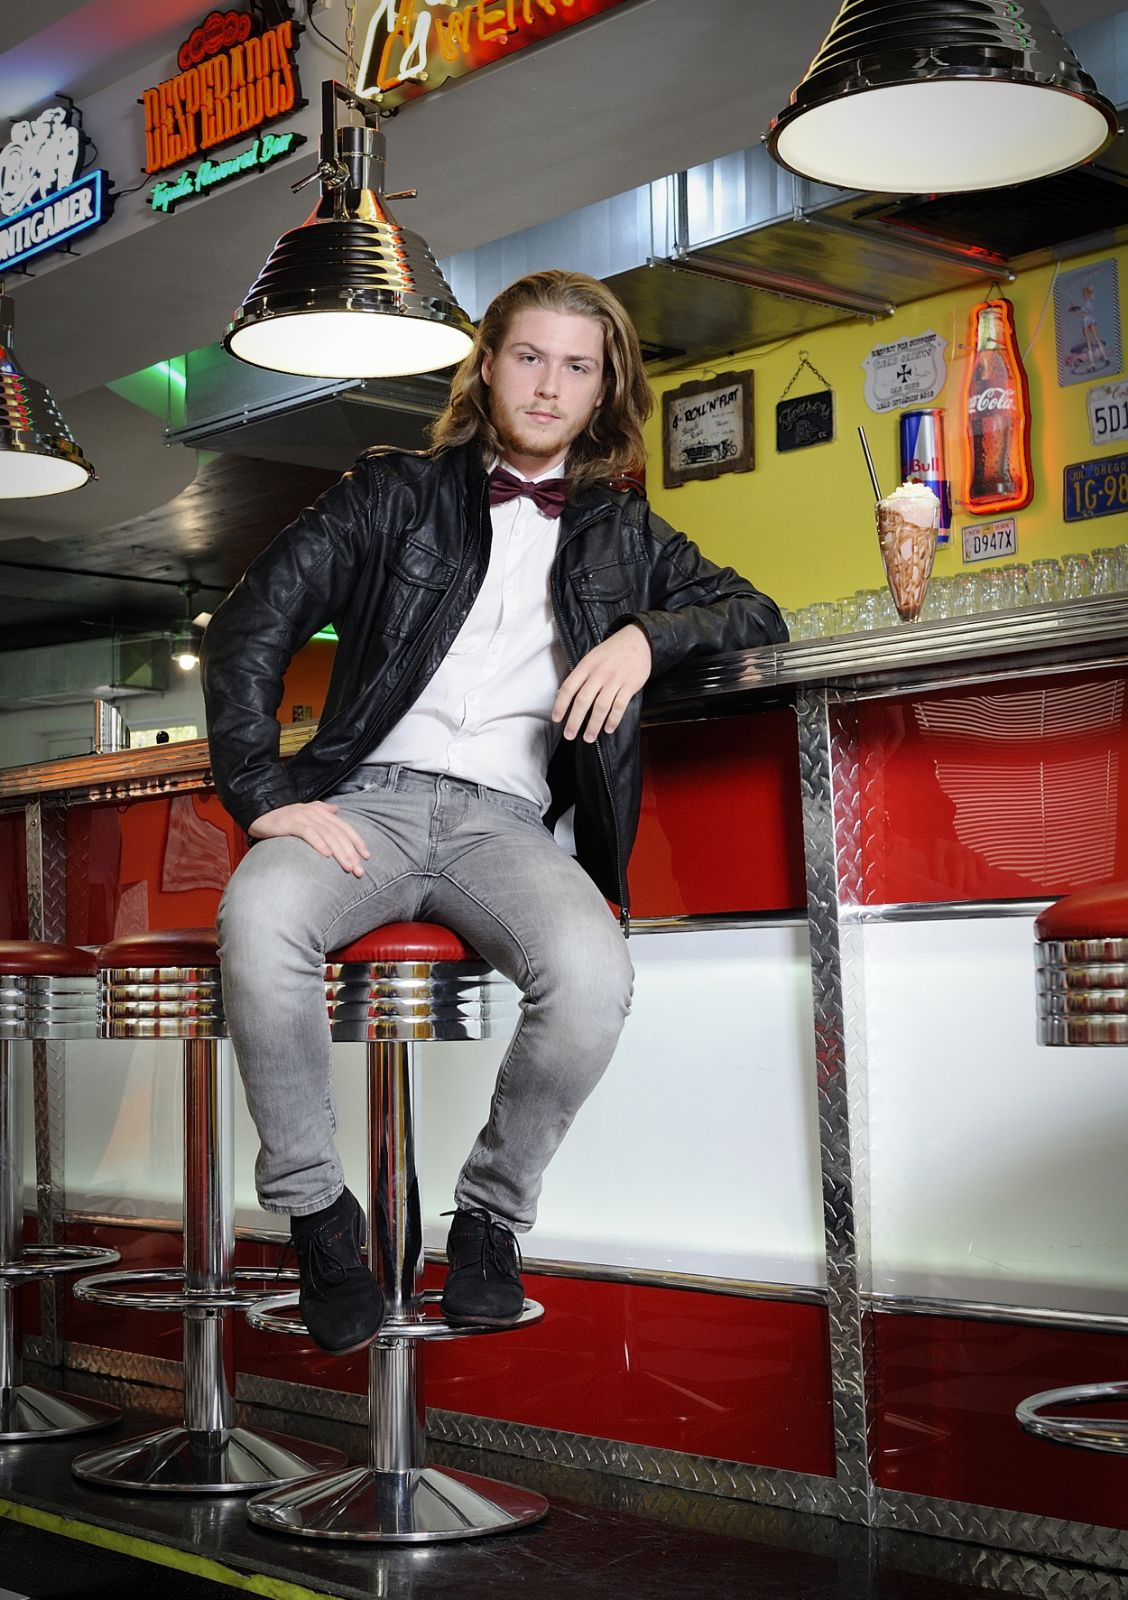
\includegraphics[width=0.35\textwidth]{Bilder/Fotos/Greistorfer}
\end{center}
\end{wrapfigure}
\mbox{}\\
\mbox{}\\
\mbox{}\\
\mbox{}\\
\mbox{}\\
\textbf{Aufgabenbereich}:\\
Webserver\\
Webclient\\
\textbf{Betreuer}:\\
Dip.-Ing. Manfred Steiner
\mbox{}\\
\mbox{}\\
\mbox{}\\
\mbox{}\\
\mbox{}\\

\subsection*{Florian Harrer}
\begin{wrapfigure}[15]{l}{0.5\textwidth}
\begin{center}
  \includegraphics[width=0.35\textwidth]{Bilder/Fotos/Harrer}
\end{center}
\end{wrapfigure}
\mbox{}\\
\mbox{}\\
\mbox{}\\
\mbox{}\\
\mbox{}\\
\mbox{}\\
\textbf{Aufgabenbereich}:\\
Java-Programm\\
\textbf{Betreuer}:\\
Dip.-Ing. Manfred Steiner
\mbox{}\\
\mbox{}\\
\mbox{}\\
\mbox{}\\
\mbox{}\\
\newpage

\subsection*{Dominik Pichler}
\begin{wrapfigure}[12]{l}{0.5\textwidth}
\begin{center}
  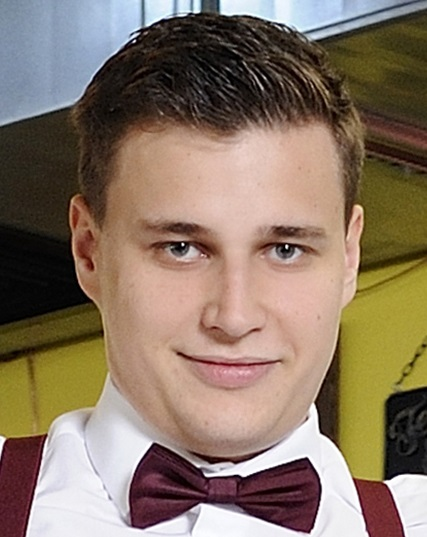
\includegraphics[width=0.35\textwidth]{Bilder/Fotos/Pichler}
\end{center}
\end{wrapfigure}
\mbox{}\\
\mbox{}\\
\mbox{}\\
\mbox{}\\
\mbox{}\\
\mbox{}\\
\textbf{Aufgabenbereich}:\\
Mechanik\\
\textbf{Betreuer}:\\
Dip.-Ing. Dr. Gerhard Pretterhofer
\mbox{}\\
\mbox{}\\
\mbox{}\\
\mbox{}\\
\mbox{}\\

\subsection*{Julian Wolf}
\begin{wrapfigure}[15]{l}{0.5\textwidth}
\begin{center}
  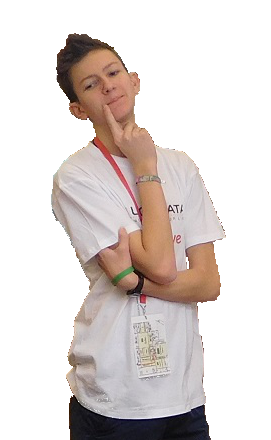
\includegraphics[width=0.35\textwidth]{Bilder/Fotos/Wolf}
\end{center}
\end{wrapfigure}
\mbox{}\\
\mbox{}\\
\mbox{}\\
\mbox{}\\
\mbox{}\\
\textbf{Aufgabenbereich}:\\
Elektrotechnik\\
Mechanik\\
\textbf{Betreuer}:\\
Otto Schuller BEd.